\documentclass[10pt,a4paper]{amsart}
\usepackage[margin=19mm]{geometry}
\usepackage{amsmath,amssymb,mathtools}
\usepackage[scr=rsfs,cal=euler]{mathalfa}
\usepackage{xfrac}
\usepackage[unicode,hidelinks,bookmarks=false]{hyperref}
\newcommand{\ie}{i.e.\ }
\newcommand{\cf}{cf.\ }
\newcommand{\resp}{respectively\ }
\newcommand{\Subsection}{\subsection}
\providecommand{\nobreakdash}{\nobreak\hbox{-}}
\setlength{\emergencystretch}{2em}
\multlinegap0pt
\usepackage{tikz}
\usepackage{amssymb}
\usepackage{mathtools}
\usepackage{xcolor}
\usepackage[shortlabels]{enumitem}
\usepackage{float}
\newtheorem{lemma}{Lemma}
\def\integers{{\mathbb{Z}}}
\def\lcm{\mathrm{lcm}}
\title{Commensurability and quasi-isometry classification for one vertex one loop tubular groups}
\author{Amy Tao}
\date{Source: arXiv:2609.05705v1 (CC BY 4.0)}
\begin{document}
\maketitle

\noindent\emph{Source and licence.} Commensurability and quasi-isometry classification for one vertex one loop tubular groups. Version arXiv:2609.05705v1 (CC BY 4.0), distributed by arXiv under the Creative Commons Attribution 4.0 International licence, http://creativecommons.org/licenses/by/4.0/, as recorded in the arXiv licence metadata for this exact version and shown on the abstract page https://arxiv.org/abs/2609.05705v1. Full licence notice: \texttt{licenses/arxiv-2609.05705-CC-BY-4.0.txt}.\par\smallskip

\noindent\textit{Editorial scope.} Counted unit: the article's lemma lemma (source0.tex lines 952--954). The article's complete original proof of it is delivered with it (source0.tex lines 955--1026, one \texttt{proof} environment of 72 lines). No mathematics is written, repaired or re-derived: the statement and the proof are the article's own lines, in the article's own notation, and no retained line is substituted or re-flowed.  No further source-local context is needed: every cross-reference of every retained line resolves inside the two delivered spans.  Nothing was omitted from any retained span, so the package carries no omission record.  No retained line contains a citation, so the wrapper carries no bibliography and no bibliography entry.  The retained lines contain the article's own diagram code, which the wrapper typesets with the standard tikz packages; no image file is delivered and the package declares no asset dependency.  Editorial formatting only, in addition: an AMS \texttt{amsart} preamble that restates the article's own declarations and macros used by the retained lines, namely the environments \texttt{lemma} on separate counters, together with the standard packages those lines need.  The retained environments print in this document as Lemma 1 in order of appearance, whereas the article prints the same items with the numbering of its own full document.  The complete native source of the article as distributed in the arXiv e-print for this exact version is bundled unchanged as \texttt{sources/209459/source0.tex}.
\begin{lemma}
    $G_{(m,0),(n,0)}$ where $\gcd(m,n)=1$ is commensurable to $G_{(km,0),(kn,0)}$ for any nonzero integer $k$. 
\end{lemma}

\begin{proof}

We first handle the case where $m=n$. Consider the map $G_{(m,0),(m,0)} \twoheadrightarrow \integers/m\integers$ sending $a \mapsto 1, b\mapsto 0, t\mapsto 0$. The kernel of this map has graph of groups structure with one vertex and $|m|$ loops, depicted in the leftmost picture below. 

\begin{tikzpicture}
\node at (0,0) (1)[left]{$\langle  a^m, b \rangle$};
\path[every node/.style={font=\sffamily\small}]
(1)   edge[in=45,out=15, loop, distance=2.5cm] node[right]  {$\langle a^m \rangle$} (1);
\path (1)   edge[in=-45,out=-15, loop, distance=2.5cm] node[right]  {} (1);
\node at (2,0) (dots) {$\vdots \hspace{0.5cm} |m|$ loops};
\node at (0.6,1.4) (out) {$a^m$};
\node at (1.5,0.5) (in) {$a^m$};
\node at (4,0) (sim) {$\simeq$};

\node at (6,0) (1)[left]{$\langle  \alpha,\beta \rangle$};
\path[every node/.style={font=\sffamily\small}]
(1)   edge[in=45,out=15, loop, distance=2.5cm] node[right]  {$\langle \alpha \rangle$} (1);
\path (1)   edge[in=-45,out=-15, loop, distance=2.5cm] node[right]  {} (1);
\node at (8,0) (dots) {$\vdots$ \hspace{0.5cm} $|m|$ loops};
\node at (6.6,1.4) (out) {$\alpha$};
\node at (7.5,0.5) (in) {$\alpha$};

\node at (10.5,0) (sim) {$\simeq$};

\node at (12,0) (1)[left]{$\langle  a,b^m \rangle$};
\path[every node/.style={font=\sffamily\small}]
(1)   edge[in=45,out=15, loop, distance=2.5cm] node[right]  {$\langle a \rangle$} (1);
\path (1)   edge[in=-45,out=-15, loop, distance=2.5cm] node[right]  {} (1);
\node at (14,0) (dots) {$\vdots$ \hspace{0.5cm} $|m|$ loops};
\node at (12.6,1.4) (out) {$a$};
\node at (13.5,0.5) (in) {$a$};
\end{tikzpicture}

Letting $\alpha=a^m, \beta=b$, we get the middle picture. But then we recognize this as isomorphic to the rightmost picture, which is the kernel of the map $G_{(1,0),(1,0)} \twoheadrightarrow \integers/m\integers$ sending $a\mapsto 0,b \mapsto 1,t\mapsto 0$. So $G_{(m,0),(m,0)}$ is commensurable to $G_{(1,0),(1,0)}$ for any $m\ne 0$, and hence to each other.


Now suppose $m\ne n$. Consider the map $G_{(km,0),(kn,0)} \twoheadrightarrow \integers/k|m-n|\integers$ sending $a\mapsto 1,b\mapsto 0, t \mapsto 0$. The kernel of this map has graph of groups structure with one vertex and $\gcd(km,k|m-n|) = |k|\gcd(m,|m-n|) = |k|\gcd(m,n)=|k|$ many loops. Note $\lcm(km,k|m-n|) = |k m|\:|m-n|$. So the edge groups have generator $(a^{km})^{|m-n|}$ and the other map goes to $(a^{kn})^{|m-n|}$. 
%(the power of $a$ is the least common multiple up to sign)
\begin{center}
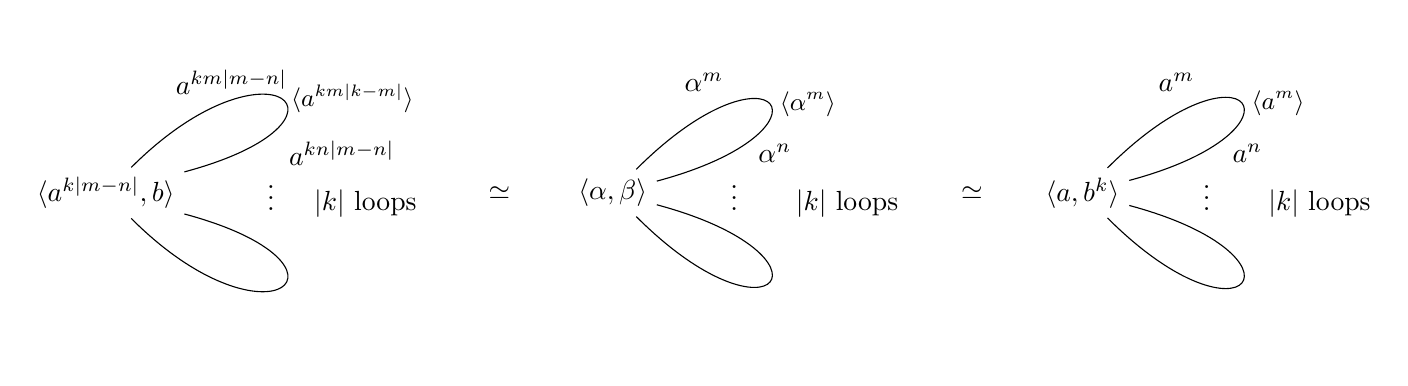
\begin{tikzpicture}
\node at (0,0) (1)[left]{$\langle  a^{k|m-n|}, b \rangle$};
\path[every node/.style={font=\sffamily\small}]
(1)   edge[in=45,out=15, loop, distance=2.5cm] node[right]  {$\langle a^{km|k-m|} \rangle$} (1);
\path (1)   edge[in=-45,out=-15, loop, distance=2.5cm] node[right]  {} (1);
\node at (2,0) (dots) {$\vdots \hspace{0.5cm} |k|$ loops};
\node at (0.6,1.4) (out) {$a^{km|m-n|}$};
\node at (2,0.5) (in) {$a^{kn|m-n|}$};
\node at (4,0) (sim) {$\simeq$};

\node at (6,0) (1)[left]{$\langle  \alpha,\beta \rangle$};
\path[every node/.style={font=\sffamily\small}]
(1)   edge[in=45,out=15, loop, distance=2.5cm] node[right]  {$\langle \alpha^m \rangle$} (1);
\path (1)   edge[in=-45,out=-15, loop, distance=2.5cm] node[right]  {} (1);
\node at (8,0) (dots) {$\vdots$ \hspace{0.5cm} $|k|$ loops};
\node at (6.6,1.4) (out) {$\alpha^m$};
\node at (7.5,0.5) (in) {$\alpha^n$};

\node at (10,0) (sim) {$\simeq$};

\node at (12,0) (1)[left]{$\langle  a,b^k \rangle$};
\path[every node/.style={font=\sffamily\small}]
(1)   edge[in=45,out=15, loop, distance=2.5cm] node[right]  {$\langle a^m \rangle$} (1);
\path (1)   edge[in=-45,out=-15, loop, distance=2.5cm] node[right]  {} (1);
\node at (14,0) (dots) {$\vdots$ \hspace{0.5cm} $|k|$ loops};
\node at (12.6,1.4) (out) {$a^m$};
\node at (13.5,0.5) (in) {$a^n$};
\end{tikzpicture}
\end{center}

Letting $\alpha=a^{k|m-n|},\beta=b$, we get the middle picture. But then we recognize that as a finite index subgroup of $G_{(m,0),(n,0)}$, namely the kernel of the map $G_{(m,0),(n,0)} \twoheadrightarrow \integers/k\integers$ sending $a \mapsto 0, b\mapsto 1, t\mapsto 0$. Therefore $G_{(km,0),(kn,0)}$ and $G_{(m,0),(n,0)}$ are commensurable. 
    
\end{proof}

\end{document}
